\chapter{Planificación}\label{chap:planif}
La planificación de un proyecto es fundamental para su correcto funcionamiento y desarrollo,
dentro de los plazos y costes establecidos. En este apartado se detallan las tareas que se
llevarán a cabo en el proyecto, así como los recursos necesarios y los plazos de ejecución.

\section{Metodología}\label{sec:metodología}
En este capítulo se aborda la metodología adoptada para el desarrollo del proyecto, fundamentada
en principios ágiles y enfocada en la entrega continua de valor. La elección de \textit{Scrum}
como marco de trabajo subraya nuestro compromiso con la adaptabilidad y la mejora continua.

La estructura de este capítulo se organiza en torno a la descripción detallada de la metodología
\textit{Scrum}, la visualización de la planificación y las estrategias de comunicación adoptadas.
A través de esta metodología, buscamos optimizar los recursos disponibles, ajustarnos a los plazos
establecidos y garantizar la calidad del producto final.

La implementación de \textit{Scrum} se complementa con herramientas de visualización y gestión de
proyectos, como los tableros de \textit{GitHub}, que facilitan la organización y seguimiento de
las tareas. Además, se pone especial énfasis en la comunicación efectiva dentro del equipo de
desarrollo y con los stakeholders, asegurando así una alineación constante con los objetivos del
proyecto.

Este enfoque metodológico no solo refleja la planificación y ejecución del proyecto, sino que
también establece las bases para una gestión eficaz, adaptativa y orientada a resultados.

\subsection{Scrum}\label{subsec:scrum}
Para la planificación del proyecto se ha escogido \textit{Scrum}, una metodología ``ágil'' que se
basa en la realización de iteraciones cortas y en la adaptación a los cambios. La metodología
\textit{Scrum} se estructura en \textit{sprints} (iteraciones cortas de una duración fija),
en las que se llevan a cabo una serie de tareas que se han planificado previamente.

El primer paso de la metodología \textit{Scrum} es la creación de un \textit{product backlog},
una lista ordenada de las tareas a realizar durante el desarrollo del producto, a partir de los
requisitos del sistema, que a su vez son una versión refinada de los requisitos iniciales del
proyecto. A partir de este \textit{product backlog} se planifican las tareas que se llevarán
a cabo en cada \textit{sprint}, de manera que sea posible cumplir con los objetivos del proyecto
en el tiempo establecido.

\subsection{Visualización de la planificación}\label{subsec:visual_planif}
Para la visualización de la planificación se ha utilizado la herramienta de gestión de proyectos
de \textit{GitHub}, que permite múltiples visualizaciones de tareas e \textit{issues} en tableros
separados.

\begin{itemize}
	\item Se utiliza un tablero de \textit{requisitos} al estilo \textit{Kanban} para visualizar
		los requisitos del proyecto y su estado, siguiendo con la metodología \textit{Scrum}.
	\item Se utiliza un \textit{roadmap} de tareas, donde se visualizan las tareas y los hitos
		del proyecto, así como su estado y sus fechas límite. Este \textit{roadmap} no está
		relacionado con la metodología \textit{Scrum}, sino que se ha creado a propósito para
		facilitar la visualización de las tareas y hitos de partes del proyecto separadas del
		desarrollo, como los apartados de la memoria o los plazos de entrega del proyecto.
\end{itemize}

\begin{minipage}{0.9\linewidth}
	\centering
	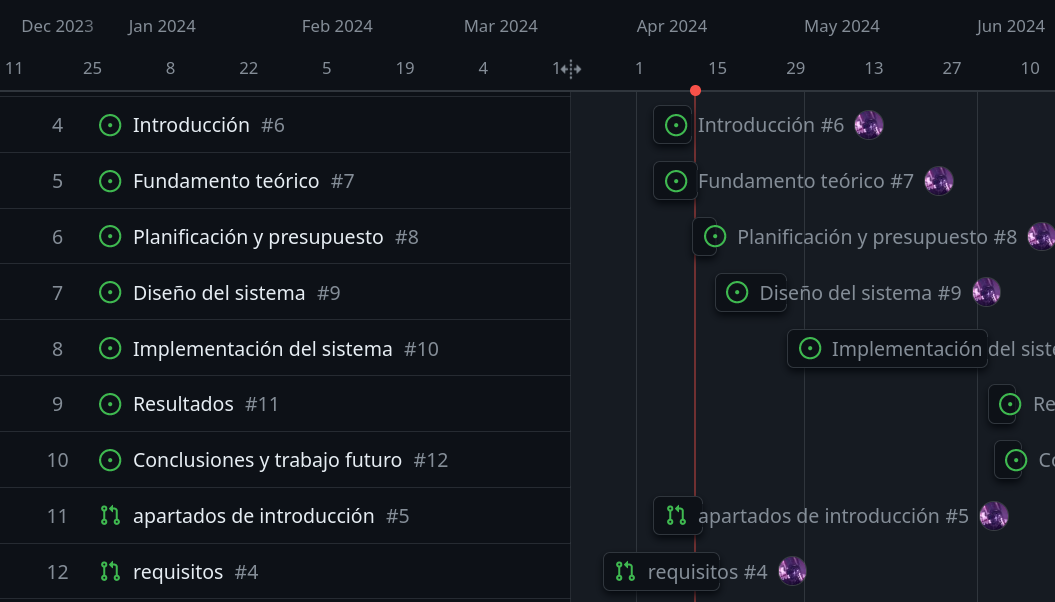
\includegraphics[width=0.95\textwidth]{roadmap.png}
	\captionof{figure}{Roadmap de tareas}
\end{minipage}

\subsection{Comunicación}\label{subsec:comunicación}
La comunicación con los tutores y con el equipo de desarrollo se considera fundamental para el
correcto desarrollo del proyecto. Puesto que el trabajo se desarrolla de manera presencial en
la oficina de la empresa, la comunicación con el equipo de desarrollo se realiza de manera
frecuente y directa, mientras que la comunicación con los tutores se realiza de manera remota
pero igual de frecuente, manteniendo el contacto mediante correo electrónico y Teams para
pedir revisiones e informar sobre el estado del trabajo en todo momento.

\subsection{Plataformas de desarrollo}\label{subsec:plataformas}
Con el objetivo de facilitar las tareas de desarrollo y cumplimentar los requisitos por parte
de la empresa, se utilizan las siguientes plataformas y herramientas de desarrollo para la
fabricación del proyecto:

\begin{itemize}
	\item \textbf{GitHub}: Plataforma de desarrollo colaborativo para el desarrollo del proyecto.
		Se utiliza para la gestión de tareas, seguimiento de desarrollo, documentación y
		colaboración.
	\item \textbf{Atlassian suite (\emph{Jira, Bitbucket})}: Suite de herramientas de gestión de proyectos
		y desarrollo colaborativo. Se utiliza para el desarrollo y documentación del proyecto de
		parte de la empresa.
	\item \textbf{Visual Studio Code}: IDE para el desarrollo del proyecto. Se utiliza para el
		desarrollo tanto del proyecto como la memoria.
	\item \textbf{\LaTeX}: Sistema de gestión de documentos para la creación de la memoria.
		Se utiliza para la creación de la memoria del proyecto.
\end{itemize}

\newpage{}
\section{Presupuesto}\label{sec:presupuesto}
